%% 
%% Copyright 2007-2020 Elsevier Ltd
%% 
%% This file is part of the 'Elsarticle Bundle'.
%% ---------------------------------------------
%% 
%% It may be distributed under the conditions of the LaTeX Project Public
%% License, either version 1.2 of this license or (at your option) any
%% later version.  The latest version of this license is in
%%    http://www.latex-project.org/lppl.txt
%% and version 1.2 or later is part of all distributions of LaTeX
%% version 1999/12/01 or later.
%% 
%% The list of all files belonging to the 'Elsarticle Bundle' is
%% given in the file `manifest.txt'.
%% 
%% Template article for Elsevier's document class `elsarticle'
%% with harvard style bibliographic references

%\documentclass[preprint,12pt,authoryear]{elsarticle}

%% Use the option review to obtain double line spacing
%% \documentclass[authoryear,preprint,review,12pt]{elsarticle}

%% Use the options 1p,twocolumn; 3p; 3p,twocolumn; 5p; or 5p,twocolumn
%% for a journal layout:
%% \documentclass[final,1p,times,authoryear]{elsarticle}
%% \documentclass[final,1p,times,twocolumn,authoryear]{elsarticle}
%% \documentclass[final,3p,times,authoryear]{elsarticle}
%% \documentclass[final,3p,times,twocolumn,authoryear]{elsarticle}
%% \documentclass[final,5p,times,authoryear]{elsarticle}
 \documentclass[final,5p,times,twocolumn, nopreprintline]{elsarticle}

%% For including figures, graphicx.sty has been loaded in
%% elsarticle.cls. If you prefer to use the old commands
%% please give \usepackage{epsfig}

%% The amssymb package provides various useful mathematical symbols
\usepackage{amssymb}
\usepackage{lipsum}
\usepackage{tikz}
\usetikzlibrary{calc,angles,positioning,babel,arrows.meta}
\usepackage{amsmath}
\usepackage[utf8]{inputenc}
%\usepackage[pdftex,active,tightpage]{preview}
%\setlength\PreviewBorder{2mm}
\usepackage{url}
\usepackage{pgfplots}
\pgfplotsset{compat=1.10}
\usepgfplotslibrary{fillbetween}
\usepackage[spanish]{babel}
%% The amsthm package provides extended theorem environments
%% \usepackage{amsthm}

%% The lineno packages adds line numbers. Start line numbering with
%% \begin{linenumbers}, end it with \end{linenumbers}. Or switch it on
%% for the whole article with \linenumbers.
%% \usepackage{lineno}

%% You might want to define your own abbreviated commands for common used terms, e.g.:
\newcommand{\kms}{km\,s$^{-1}$}
\newcommand{\msun}{$M_\odot}
\newcommand{\toplrarr}[1]{\overset{\text{\scriptsize$\leftrightarrow$}}{#1}}
\numberwithin{equation}{section}
%\journal{Astronomy $\&$ Computing}

\begin{document}

\begin{frontmatter}

%% Title, authors and addresses

%% use the tnoteref command within \title for footnotes;
%% use the tnotetext command for theassociated footnote;
%% use the fnref command within \author or \affiliation for footnotes;
%% use the fntext command for theassociated footnote;
%% use the corref command within \author for corresponding author footnotes;
%% use the cortext command for theassociated footnote;
%% use the ead command for the email address,
%% and the form \ead[url] for the home page:
%% \title{Title\tnoteref{label1}}
%% \tnotetext[label1]{}
%% \author{Name\corref{cor1}\fnref{label2}}
%% \ead{email address}
%% \ead[url]{home page}
%% \fntext[label2]{}
%% \cortext[cor1]{}
%% \affiliation{organization={},
%%            addressline={}, 
%%            city={},
%%            postcode={}, 
%%            state={},
%%            country={}}
%% \fntext[label3]{}

\title{Caracterización estructural y óptica de una muestra policristalina de $\text{La}_2\text{O}_3$.}

%% use optional labels to link authors explicitly to addresses:
%% \author[label1,label2]{}
%% \affiliation[label1]{organization={},
%%             addressline={},
%%             city={},
%%             postcode={},
%%             state={},
%%             country={}}
%%
%% \affiliation[label2]{organization={},
%%             addressline={},
%%             city={},
%%             postcode={},
%%             state={},
%%             country={}}

\author[first]{Sebastián Carrillo Mejía}

\author[first]{Andrés Felipe Riaño Quintanilla}


\author[first]{Santiago Julio Dávila}
\affiliation[first]{organization={Instituto de Física, Universidad de Antioquia},%Department and Organization
            city={Medellín},
            state={Antioquia},
            country={Colombia}}



%%Graphical abstract
%\begin{graphicalabstract}
%\includegraphics{grabs}
%\end{graphicalabstract}

%%Research highlights
%\begin{highlights}
%\item Research highlight 1
%\item Research highlight 2
%\end{highlights}

\begin{abstract}

\end{abstract}

\begin{keyword}

\end{keyword}

\end{frontmatter}

%\tableofcontents

%% \linenumbers

%% main text

\section{Introducción}

\section{Marco teórico} 

\subsection{Difracción de Rayos X}

Se conoce como \emph{difracción de rayos X} (DRX) a la dispersión elástica de fotones de rayos X producida por los átomos de una red periódica \cite{chatterjee2000x}, como se muestra en la figura \ref{fig:bragg}.

\begin{figure}[h!]
\centering
\begin{tikzpicture}[dot/.style={circle,draw,fill=black,minimum size=5}]

%\draw[
%  help lines,
%  line width=0.1pt,
%  gray!30,
%] (-2, -6) grid[step={($(0.25, 0.25) - (0, 0)$)}] (6, 2);
%\draw[
%  help lines,
%  line width=0.1pt,
%  gray,
%] (-2, -6) grid[step={($(1, 1) - (0, 0)$)}] (6, 2);

\draw[fill=cyan, fill opacity=0.5] (0,0)--(0,-1)--(0.433,-0.75) -- cycle;
\draw[fill=cyan, fill opacity=0.5] (0,0)--(0,-1)--(-0.433,-0.75) -- cycle;

\draw (-2,0) -- (2,0);
\draw (-2,-1) -- (2,-1);
\draw (-2,-2) -- (2,-2);

  \foreach \x in {-2,...,2}
    {\foreach \y in {-2,...,0} 
       \node[mark size=2pt,color=black] at (\x,\y) {\pgfuseplotmark{*}};
	 \draw (\x,-2) -- (\x,0);}
	 
\draw[red] plot[domain=0:2.309, samples=100]  ({0.866*\x-0.5*0.25*sin(2*\x*pi r)},{0.5*\x+0.866*0.25*sin(2*\x*pi r)});
\draw[red] plot[domain=-2.309:0, samples=100]  ({0.866*\x+0.5*0.25*sin(2*\x*pi r)},{-0.5*\x+0.866*0.25*sin(2*\x*pi r)});
\draw[red] plot[domain=0:2.309, samples=100]  ({0.866*\x-0.5*0.25*sin(-2*\x*pi r)},{0.5*\x+0.866*0.25*sin(-2*\x*pi r)-1});
\draw[red] plot[domain=-2.309:0, samples=100]  ({0.866*\x+0.5*0.25*sin(-2*\x*pi r)},{-0.5*\x+0.866*0.25*sin(-2*\x*pi r)-1});

\draw[thick, red] (-2,1.1545)--(0,0);
\draw[thick, red] (-2,0.1545)--(0,-1);

\draw[<->] (-1.25,-2)-- node[left] {$d$}(-1.25,-1);

\draw[-stealth,thick, red] (0,0)--(2,1.1545);
\draw[-stealth,thick, red] (0,-1)--(2,0.1545);

\draw (1,0) arc (0:30:1) node[midway,right] {$\theta$};

\draw[fill=cyan, fill opacity=0.5] (3.5,-2)--(3.5,1)--(4.799,-1.25) -- cycle;
\draw[thick,red] (3.5,-2)--(4.799,-1.25) node [midway,below right] {$d\sin\theta$};

%\draw[red] plot[domain=0:1.5, samples=50]  ({0.866*\x+0.5*0.5*sin(\x*pi/1.5 r)+3.5},{0.5*\x-0.866*0.5*sin(\x*pi/1.5 r)-2});

\draw[|<->|] (3.25,-2)-- node[left] {$d$}(3.25,1);

\draw (3.5,0) arc (-90:-60:1) node[midway, below] {$\theta$};

\end{tikzpicture}

\caption{Condición de interferencia constructiva para DRX. Aquí, $\theta$ es el ángulo de incidencia con respecto al plano cristalográfico y $d$ es la distancia interplanar.}
\end{figure} \label{fig:bragg}

Para obtener una interverencia constructiva en la pantalla de observación se requiere que las ondas estén en fase, esto es, que el desfase inducido por la diferencia de camino óptico, $\Delta\phi=k\Delta r$, sea un múltiplo entero de $2\pi$ \cite{hecht2012optics}, donde $k=2\pi/\lambda$ es el número de onda. De la figura \ref{fig:bragg} es evidente que la diferencia de camino óptico es $\Delta r = 2d\sin\theta$, de modo que la condición para interferencia constructiva es

\begin{equation}
n\lambda = 2d_{hkl}\sin\theta. \label{eq:bragg}
\end{equation}

La ecuación \ref{eq:bragg} se conoce como \emph{ley de Bragg}, y es válida para $\lambda\leq 2d_{hkl}$. Se ha adoptado la notación $d_{hkl}$ para la distancia interplanar, donde $hkl$ son los \emph{índices de Miller} del plano cristalográfico, que caracterizan su orientación. Para un conjunto de planos $\{hkl\}$ con distancia interplanar fija $d_{hkl}$ solo se obtiene interferencia constructiva para ciertos valores de $\theta$ \cite{kittel2018introduction}, esto gráficamente se evidencia como un conjunto de deltas de Dirac en los valores de $\theta$ para los cuales se satisface la ley de Bragg, y a partir del cual se pueden obtener los parámetros de red del cristal \cite{ds1989simple}.\\

Si se tiene una muestra policristalina, estos picos presentan un ensanchamiento debido a diferentes efectos, siendo de particular interés los ensanchamientos por \emph{tamaño medio del cristalito} y \emph{microtensiones}, que pueden modelarse a través de la ecuación

\begin{equation}
B_{hkl}\cos\theta=\dfrac{K\lambda}{L}+\epsilon(4\sin\theta) \label{eq:wh1}
\end{equation}

donde $B_{hkl}$ es el ancho a media altura del pico correspondiente al plano con índices $hkl$, $L$ es el tamaño medio del cristalito, $\epsilon$ es la deformación del cristal y $K$ es la constante de Scherrer, que suele tomarse aproximadamente igual a 1. Si se definen $X=4\sin\theta$ y $Y=B_{hkl}\cos\theta$ en a ecuación \ref{eq:wh1}, se pueden obtener el tamaño del cristalito y la deformación media a través de un ajuste lineal de la forma $Y=b+mX$

\begin{align}
L=\dfrac{K\lambda}{b}\\
\epsilon=m,
\end{align} \label{eq:wh2}

este proceso se conoce como el \emph{método de Williamson-Hall} \cite{himabindu2021microstructural}.


\subsection{Espectrofotometría}

\section{Metodología}

\subsection{Difracción de rayos X}

La obtención del espectrograma se obtuvo en el \textit{Laboratorio de Difracción de Rayos X} de la Universidad de Antioquia. Allí se preparó una muestra en polvo de óxido de lantano $\text{La}_2\text{O}_3$ para ser analizada con el difractómetro del laboratorio. La muestra debe ser pasante malla 100 para garantizar que la distribución de tamaño de partículas sea homogénea. La muestra es entonces disupesta en el portamuestras y compactada, garantizando una superficie plana, para poder ser insertada en el difractómetro. El difractograma obtenido se analizó usando el software \textit{VESTA}, \textit{FullProf Suite} y Python, donde se comparó con los datos obtenidos de la base de datos \textit{Crystallographic Open Database (COD)} \cite{zachariasen1926kristallstruktur}, para obtener los parámetros de red del cristal y se utilizaron los datos de los picos del difractograma para obtener el tamaño del cristalto y los esfuerzos internos de la estructura policristalina a través del método de Williamson-Hall descrito en la sección interior.

\section{Resultados y discusión}

\subsection{Difracción de rayos X}

La figura \ref{fig:rawxrd} muestra los datos sin procesar, junto con los datos de fondo, extraídos con el software \textit{FullProf Suite} y ajustados a una exponencial decreciente para posteriormente ser restados del difractograma.

\begin{figure}[h!]

\centering
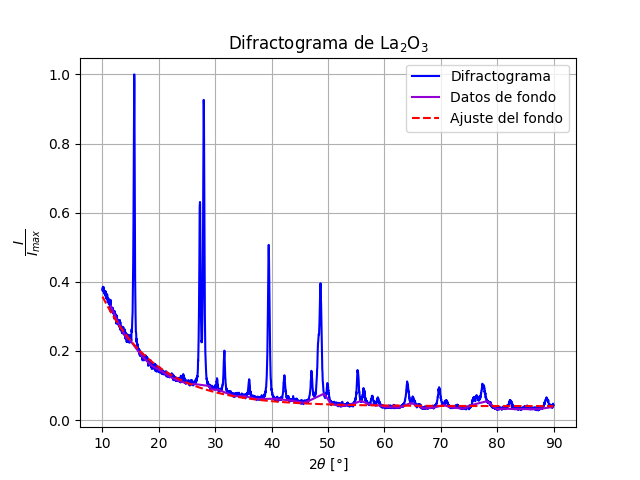
\includegraphics[width=0.8\columnwidth]{../raw_xrd.png} \label{fig:rawxrd}
\caption{Difractograma obtenido de la medición y datos de fondo.}
\end{figure}

El difractograma sin los datos de fondo es entonces comparado con los datos de COD para identificar los índices de Miller de los picos de difracción. Se consideraron solamente los picos más promientes y se tomó como referencia la intensidad relativa al máximo para la identificación de los índices con los de los picos de la base de datos y los índices reportados en la literatura \cite{kabir2018influence}, obteniendo:

\begin{figure}[h!]

\centering
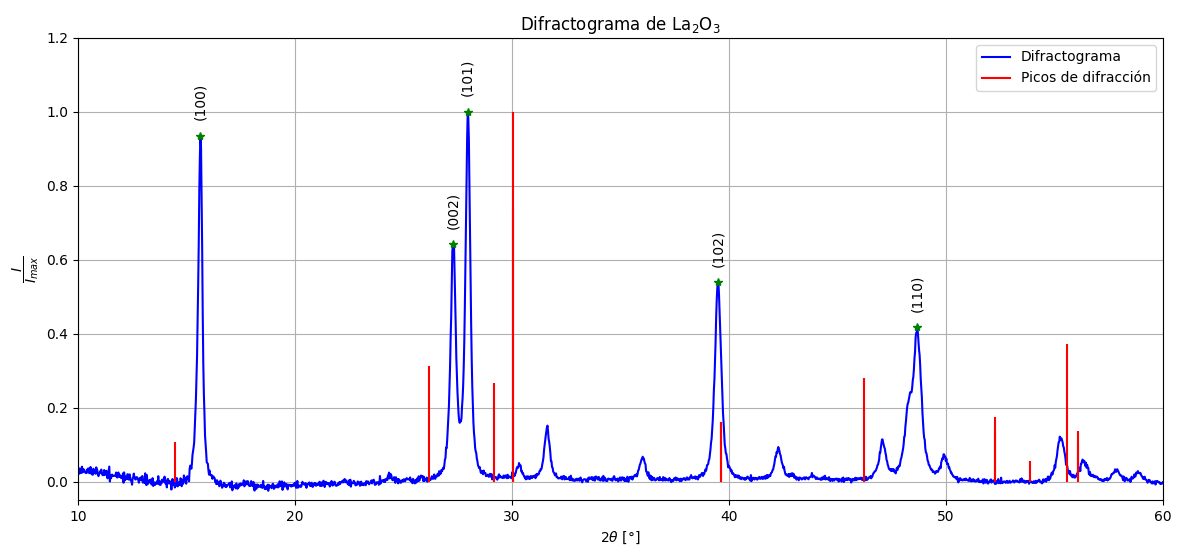
\includegraphics[width=\columnwidth]{../peaks.png} \label{fig:filtxrd}
\caption{Difractograma sin el ruido de fondo y datos de COD.}
\end{figure}

Estos datos fueron procesados con el software \textit{VESTA} para obtener los parámetros de red y una imagen tridimensional de la molécula. Los parámetros de red obtenidos son:

\begin{align*}
&a=b=3.957~\text{\r{A}},~c=6.138~\text{\r{A}}\\
&\alpha=\beta=90^\circ,~\gamma=120^\circ
\end{align*}

Estos valores para los parámetros de red son característicos de una estructura hexagonal \citep{kittel2018introduction}. En la figura \ref{fig:molecule} se observa el modelo molecular tridimensional del $\text{La}_2\text{O}_3$.


\begin{figure}[h!]
\centering
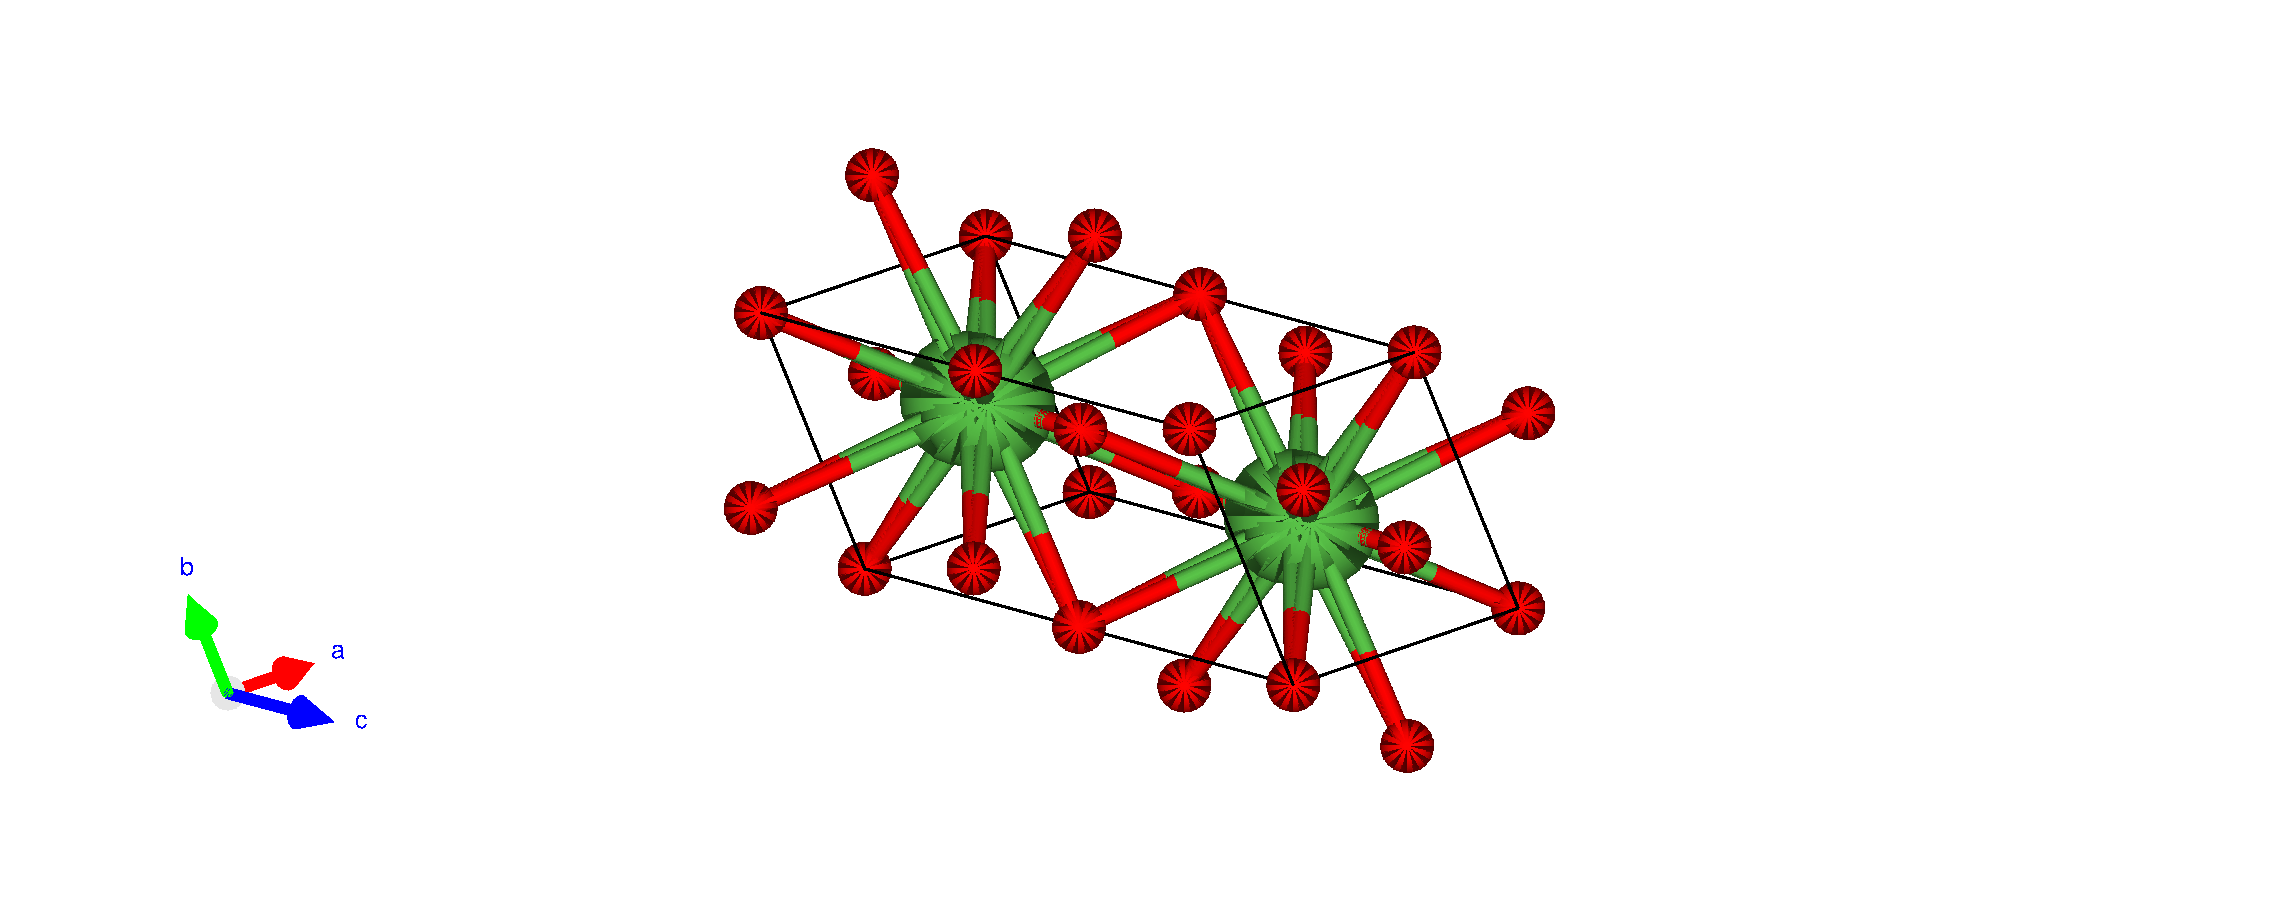
\includegraphics[width=0.8\columnwidth]{../4102405.pdf} \label{fig:molecule}
\caption{Modelo molecular del óxido de lantano. En verde se observan los átomos de lantano, en rojo los átomos de oxígeno.}
\end{figure}

Se obtuvieron además los planos cristalográficos en el modelo molecular, que se muestran en la figura \ref{fig:planes}.

\begin{figure}[h!]
\centering
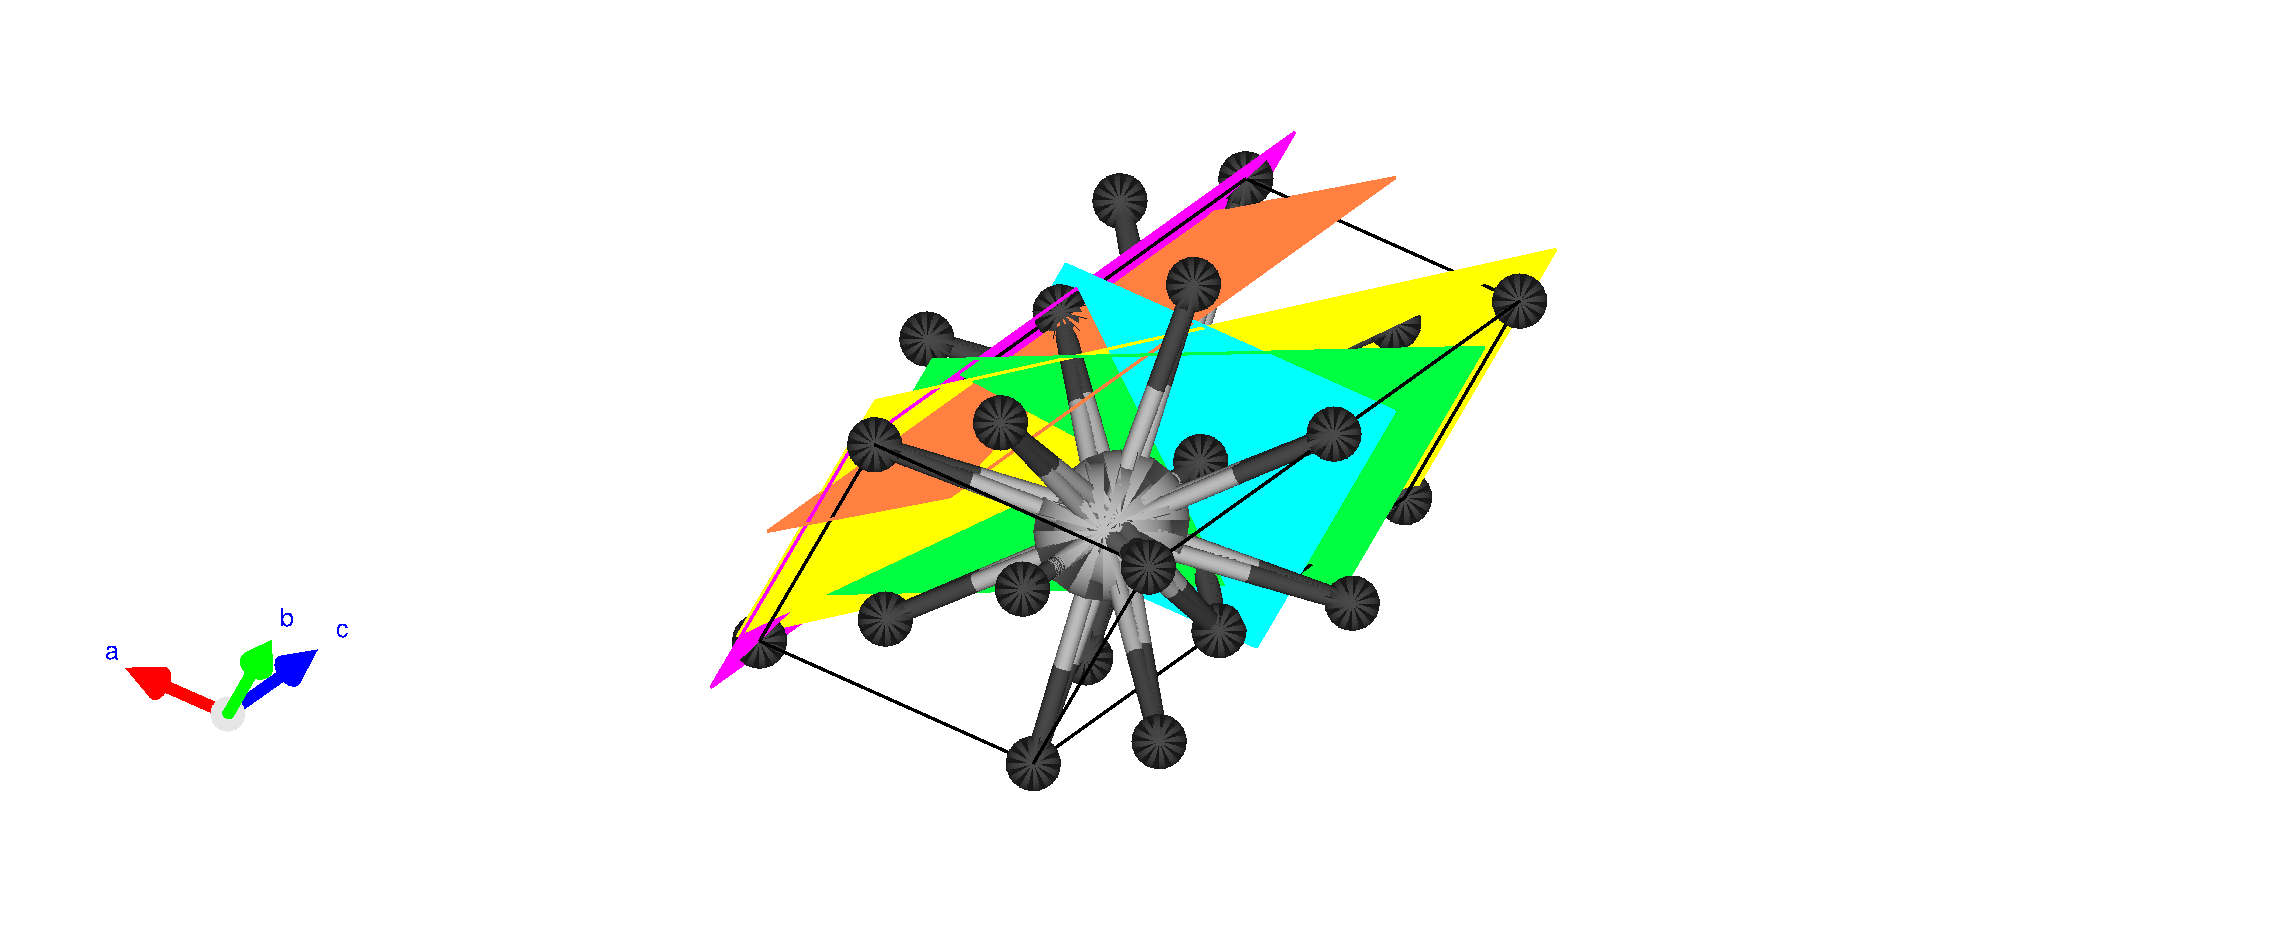
\includegraphics[width=0.8\columnwidth]{../4102405_planes.pdf} \label{fig:planes}
\caption{Planos cristalográficos en el modelo molecular del óxido de lantano. En rosado se observa el plano [100], en azul el plano [002], en amarillo el plano [101], en verde el plano [102], en naranja el plano [110].}
\end{figure}

Finalmente, con la función \texttt{peak\_widths} de la librería \texttt{scipy.signal} de Python se obtuvieron los anchos a media altura, que con las posiciones angulares de los picos se pueden ajustar a la ecuación \ref{eq:wh1} y con las ecuaciones \ref{eq:wh2} se obtienen los valores del tamaño de cristalito y el esfuerzo interno medio de la muestra analizada:

\begin{align*}
L=(39.8\pm0.1)~\text{\r{A}}\\
\epsilon=(0.3\pm0.1)
\end{align*}

El ajuste al método de Williamson-Hall se muestra en la figura \ref{fig:wh}.

\begin{figure}[h!]
\centering
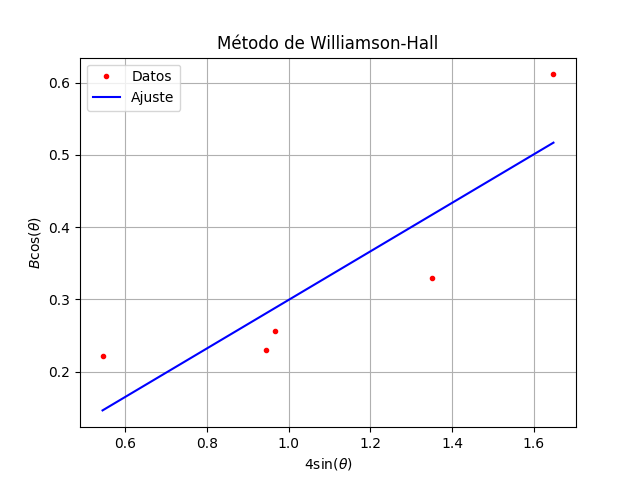
\includegraphics[width=0.8\columnwidth]{../wh.png} \label{fig:wh}
\caption{Ajuste de Williamson-Hall para el óxido de lantano.}
\end{figure}

\section{Conclusión}

\bibliographystyle{unsrt} 
\bibliography{example.bib}
%
%\bibliography{bibliography.bib}

%% else use the following coding to input the bibitems directly in the
%% TeX file.

%%\begin{thebibliography}{00}

%% \bibitem[Author(year)]{label}
%% For example:

%% \bibitem[Aladro et al.(2015)]{Aladro15} Aladro, R., Martín, S., Riquelme, D., et al. 2015, \aas, 579, A101

%%\end{thebibliography}

\end{document}

\endinput
%%
%% End of file `elsarticle-template-harv.tex'.
